\documentclass{beamer}
\usepackage{graphicx}
\usepackage[utf8]{inputenc} 
\usepackage[ngerman]{babel}

\usetheme{Warsaw}


\title{Validierung - NET-WizHearts}
\author{Patrick Kubin - Team 8}
\date{\today}

 
\begin{document}
\maketitle
\frame{
	\frametitle{Inhaltsverzeichnis}
	\tableofcontents
}
 
\section{Neuerungen}
\begin{frame}
 	\frametitle{Neuerungen}
	\ Was hat sich noch geändert?
  	\begin{itemize}
 	 	\item Überarbeitung des Spielendes
		\item Defensiver Modus
  	 	\item Steigerung der Bedienbarkeit
		\begin{itemize}
			\item View Elemente
			\item Timer für Ablagestapel
  	 		\item Kartensortierung
 	 		\item Rundenanzeige
		\end{itemize}
	\end{itemize}
\end{frame}

\section{Zahlen und Fakten zu NET-WizHearts}
\begin{frame}
	\frametitle{Überblick}
	\ Klassen in Net-WizHearts
	\begin{itemize}
		\item 229 Klassen insgesamt
		\item 114 Kernklassen
		\item 68 anonyme Klassen
		\item 42 Testklassen
		\item 5 MockObjekte
	\end{itemize}
\end{frame}

\begin{frame}
  	\frametitle{Überblick}
	\ Lines of Code in NET-WizHearts 
  	\begin{itemize}
		\item 18611 Zeilen gesamt
		\item 3675 Zeilen JavaDoc
		\item 14936 Zeilen Code
		\item 7811 Zeilen Production Code
		\item 7125 Zeilen Testcode in 295 Testfällen
		\item Code-Testcode Verhältnis ca. 1.1:1 
	\end{itemize}	
\end{frame}

\section{Line- und Branch-Coverage}
\begin{frame}
  	\frametitle{Coverage}
	\ Wie wurde getestet?
  	\begin{itemize}
		\item Coverage der View durch interaktive Tests
			\begin{itemize}
				\item Beinhaltet die Pflichtenheft Testfälle
				\item Auswertung durch EclEmma
			\end{itemize}
		\item Coverage der Kernklassen durch JUnit Tests
			\begin{itemize}
				\item Auswertung durch Cobertura
			\end{itemize}
	\end{itemize}
\end{frame}
\begin{frame}
  	\frametitle{Interaktiv}
  	\makebox[\textwidth]{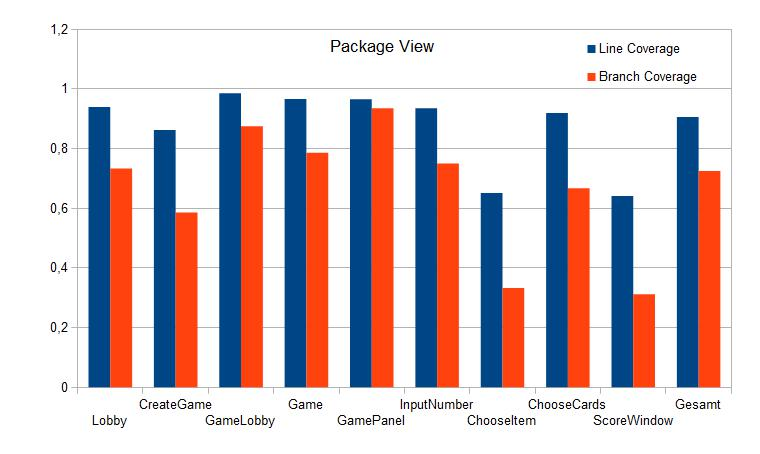
\includegraphics[scale=0.45]{images/view_interaktiv}}
\end{frame}
\begin{frame}
  	\frametitle{Interaktiv}
  	\makebox[\textwidth]{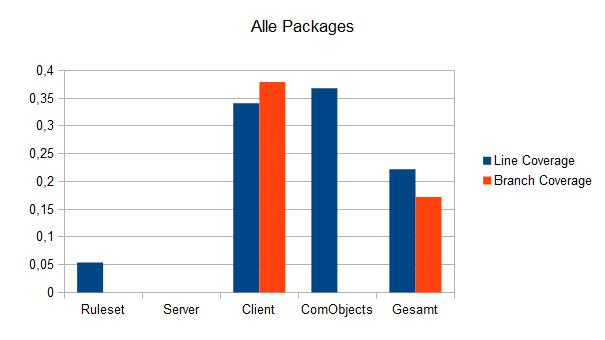
\includegraphics[scale=0.6]{images/packages_interaktiv}}
\end{frame}
\begin{frame}
  	\frametitle{JUnit}
  	\makebox[\textwidth]{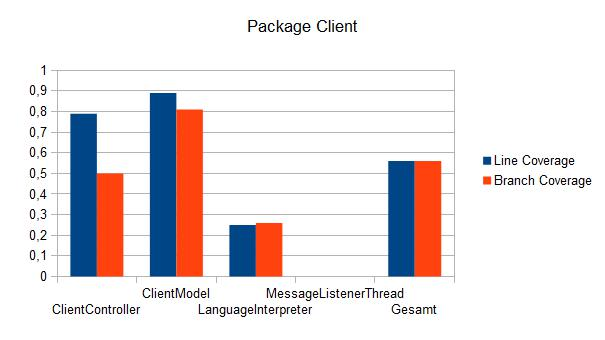
\includegraphics[scale=0.6]{images/client_junit}}
\end{frame}
\begin{frame}
  	\frametitle{JUnit}
  	\makebox[\textwidth]{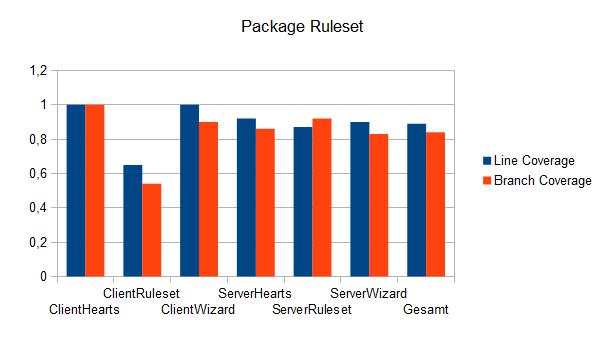
\includegraphics[scale=0.6]{images/ruleset_junit}}
\end{frame}
\begin{frame}
  	\frametitle{JUnit}
  	\makebox[\textwidth]{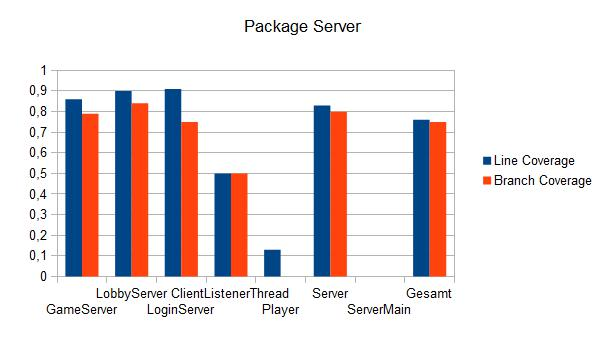
\includegraphics[scale=0.6]{images/server_junit}}
\end{frame}
\begin{frame}
  	\frametitle{JUnit}
  	\makebox[\textwidth]{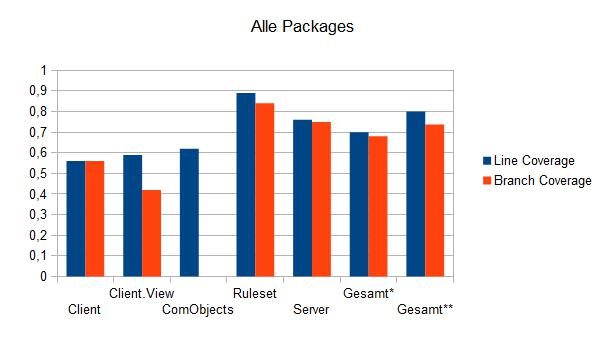
\includegraphics[scale=0.6]{images/all_packages}}
\end{frame}

\section{Korrektheitstests}
\begin{frame}
  	\frametitle{Code-Analyse mit FindBugs}
  	\begin{itemize}
		\item Fehler in Hearts Regelwerk gefunden
		\item Diverse Code Warnungen berücksichtigt
	\end{itemize}
\end{frame}
\begin{frame}
  	\frametitle{Beta-Test}
	\ Wie Vertrauen in die Software gewinnen?
	\begin{itemize}
		\item Test im Verwandtenkreis
		\item Offener Beta-Test mit bis zu 15 Spielern über das Internet
		\begin{itemize}
			\item Meldungen prüfen Zeitintensiv
			\item Falschmeldungen
		\end{itemize}
	\end{itemize}
\end{frame}
\begin{frame}
  	\frametitle{Resultate}
	\ Wichtigste Erkenntnisse aus dem Beta-Test
	\begin{itemize}
		\item Defensiver Modus
		\item Begrenzung der Länge von Spielernamen
		\item Trimmen von Blankets im Spielernamen
		\item Rundenanzeige
		\item Überarbeiten des Handbuchs
	\end{itemize}
\end{frame}

\section{Belastungstests}
\begin{frame}
  	\frametitle{Profiling}
	\ Wie wurde getestet?
  	\begin{itemize}
		\item Testumgebung
		\begin{itemize}
			\item Prozessor Intel(R) Core(TM) i5-2410M 2.30 GHz
			\item DDR3 RAM
			\item Windows 7 64 Bit
		\end{itemize}
  		\item JUnit Testfälle mit MockObjekte
		\item JProfiler
  	\end{itemize}
\end{frame}
\begin{frame}
	\frametitle{Profiling}
	\makebox[\textwidth]{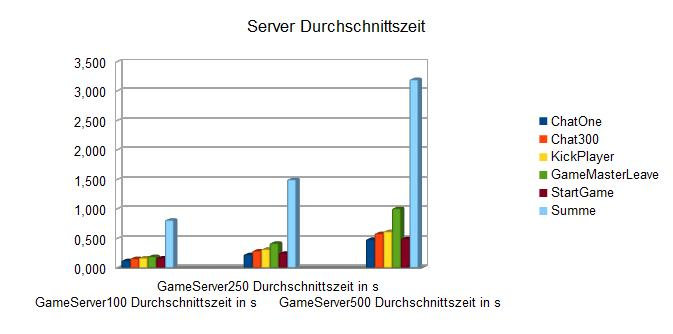
\includegraphics[scale=0.5]{images/zeit}}
\end{frame}
\begin{frame}
	\frametitle{Profiling}
	\makebox[\textwidth]{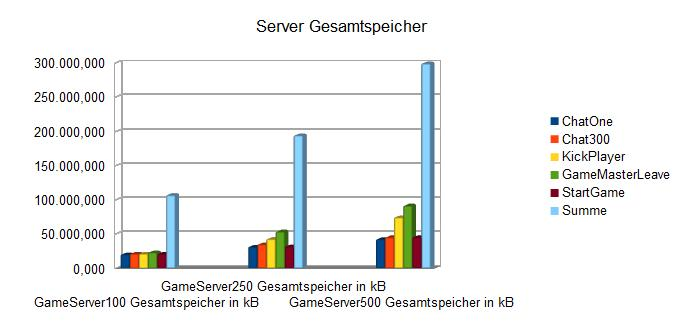
\includegraphics[scale=0.5]{images/speicher}}
\end{frame}
\begin{frame}
	\frametitle{Ende}
	\makebox[\textwidth]{
\includegraphics[scale=0.5]{images/ende}}
\end{frame}

\end{document}


